\section{Implementation}

We have implemented the keep-alive and the provisioning policies as part of our FaasCache framework built on top of OpenWhisk (Figure~\ref{fig:sys}). 

\begin{figure}[t]
  \centering
  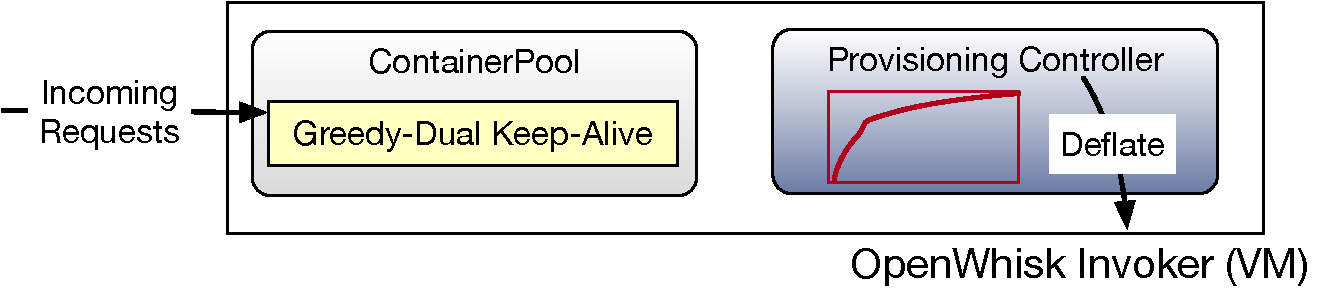
\includegraphics[width=0.8\textwidth]{faascache/faas-keepalive-20/figures/faascache.pdf}
  \caption{FaasCache system components. We build on OpenWhisk and augment it with new keep-alive policies and a provisioning controller. }
  \label{fig:sys}
\end{figure}

\noindent \textbf{Keep-Alive.}
FaasCache replaces the default OpenWhisk TTL-based keep-alive policy with the Greedy-Dual-Size-Frequency approach. 
For each initialized container, we assign and maintain the keep-alive prioritized ContainerPool, which is only a 100-line Scala modification. 
%Initialized containers are managed by the ContainerPool.
%\emph{Interesting aspects of priority calculation?} How is size, clock, frequency, cost, etc. computed? How does the impl differ from the idealized description? 
Each invocation of a function (OpenWhisk action) in ContainerPool records the launch time and when results are returned.


If the container was prewarmed before the invocation arrived, we record it as the function's warm runtime.
For new functions, the initialization overhead is captured and assumed to be the worst-case runtime until a warmed invocation is recorded. % is approximated as the minimum overhead of Docker and OpenWhisk's Python runtime initialization.
In the subsequent invocations, the initialization overhead is computed by subtracting the cold from the warm time. 
%Otherwise it was a cold start.
%The maximum cold and warm runtimes are kept per function to compute the priority.
%Size is simply the number of megabytes of memory OpenWhisk preallocates to the action's container, and
The function's frequency and clock value are updated with each request.
If the last container of a function is evicted, its cold and warm runtimes are stored and used to compute priority for its future invocations. 
%
To preserve the invocation fast-path, the ContainerPool is not kept sorted by priority. 
%Priorities are computed when an eviction needs to be made to reclaim memory.
Instead, it is sorted by priorities only during evictions, when the lowest priority container(s) are terminated.
%
We batch eviction operations to optimize the slow-path: we evict multiple containers to reach a certain free resource threshold (1000 MB is the current default). 

%rev 1
In the future, we intend to implement a similar design that is found in the Linux kernel page eviction. A separate thread (analogous to kswapd) can be used to periodically sort the containerpool list and asynchronously evict containers, so that eviction is not on the critical path. 

%All of an action's containers share one priority, regardless of the last time each ran an invocation.

% \prat{How are the values inferred?}
% New functions always replace old functions in the ContainerPool, so the priority of newly inserted containers doesn't matter. 
% After the second invocation of a function, its initialization overhead is inferred as the difference between the cold (first) and warm (subsequent) invocations. 
% Memory usage of the container is gathered via {\em Docker stats?\/}.



\noindent \textbf{Provisioning.}
For the static provisioning, we compute the reuse distance distribution for a given workload trace, and assume stationarity --- that it will be applicable on similar future workloads. 
We compute the reuse distances conventionally, by examining all reuse-sequences.
The dynamic provisioning controller runs periodically (every 10 minutes), to deflate or inflate the VM size, if the cold start rate deviates from the target significantly (by more than 30\%).
When the VM has to be shrunk, we use cascade deflation~\cite{deflation-eurosys19}.
We shrink the ContainerPool first, and reclaim the free memory using guest OS-level memory hot-unplug and hypervisor-level page swapping. 
%This approach is based on cascade deflation proposed in~\cite{deflation-eurosys19}. 

%Optimizations such as SHARDS that can significantly reduce the running time by sampling a small fraction of the functions, were found to be inadequate due to the wide disparity in the function sizes.
%The efficacy of sampling based techniques like SHARDS has mainly been empirically established only for fixed-sized objects. 


\noindent \textbf{Keep-alive Simulator.}
We have implemented a trace-driven discrete event simulator for implementing and validating different keep-alive policies.
Our simulator is written in Python in about 2,000 lines of code, and implements the various variants described in Section~\ref{subsec:variants}. 
It allows us to determine the cache hit ratios and the cold start overheads for different workloads and memory sizes.
Additionally, it also implements the static and dynamic provisioning policies for adjusting server size.

%%% Local Variables:
%%% mode: latex
%%% TeX-master: "paper"
%%% End:
